\documentclass[xcolor=table]{beamer}

\usepackage{booktabs}
\usepackage{hyperref}
\usepackage[table]{xcolor}
\usepackage{tikz}

\setbeamertemplate{navigation symbols}{}%remove navigation symbols

\title{Best Responses}
\subtitle{Game Theory}
\author{Vincent Knight}
\date{}

\tikzstyle{level 1}=[level distance=3.5cm, sibling distance=3.5cm]
\tikzstyle{level 2}=[level distance=3.5cm, sibling distance=2cm]
\tikzstyle{player} = [text width=4em, draw, text centered, rectangle, fill=blue!20, inner sep=1pt]
\tikzstyle{nature} = [minimum width=3pt,circle,  draw, fill=red!20, inner sep=1pt]
\tikzstyle{end} = [circle, minimum width=3pt, fill, inner sep=0pt, right]
\tikzstyle{dot} = [draw,shape=circle,fill=blue]

\begin{document}

\frame{\titlepage}


\frame{
\begin{center}
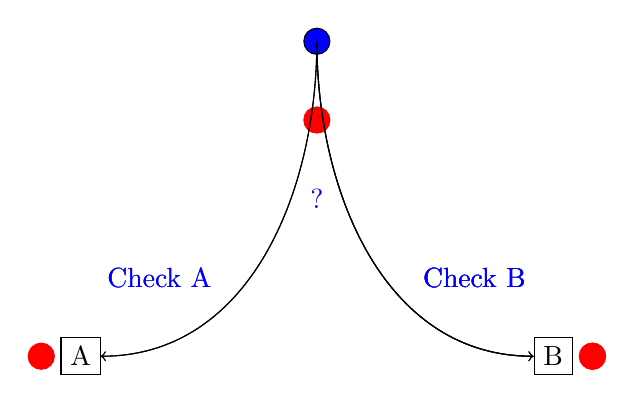
\begin{tikzpicture}

\node at (0,0) [dot] {};
\only<1>{
\node at (0,-1) [dot, red] {};}
\onslide<2->{
\node (A) at (-3,-4) [rectangle, draw] {A};
\node (B) at (3,-4) [rectangle, draw] {B};}


\onslide<2>{
\node (a) at (-2,-3) [blue] {Check A};
\node (b) at (2,-3) [blue] {Check B};
\draw (0,0) edge [out=-90, in=180, ->] (B);
\draw (0,0) edge [out=-90, in=0, ->] (A);
\node at (0,-2) [blue] {?};}

\onslide<3-4>{
\node (a) at (-2,-3) [blue] {Check A};
\draw (0,0) edge [out=-90, in=0, ->] (A);}

\onslide<4>{
\node at (3.5,-4) [dot, red] {};}

\onslide<5>{
\node at (3.5,-4) [dot, red] {};
\node (b) at (2,-3) [blue] {Check B};
\draw (0,0) edge [out=-90, in=180, ->] (B);}

\onslide<6>{
\node at (-3.5,-4) [dot, red] {};
\node (b) at (2,-3) [blue] {Check B};
\draw (0,0) edge [out=-90, in=180, ->] (B);}

\end{tikzpicture}
\end{center}
}

\frame{
\begin{center}
\begin{tikzpicture}
\node at (0,0) { $\begin{pmatrix}(1,-1)&(-1,1)\\ (-1,1)&(1,-1)\end{pmatrix}$};

\node (A) at (2,2) [color=red] {Hide A};
\draw (A) edge [color=red, out=90, in=90, ->, very thick] (-.6,.5) ;

\node (B) at (3,1) [color=blue] {Hide B};
\draw (B) edge [color=blue, out=-90, in=90, ->, very thick] (.8,.5) ;

\node (D) at (-3,-2) [color=red] {Check A};
\draw (D) edge [color=red, out=90, in=180, ->, very thick] (-1.5,.25) ;

\node (C) at (-2,-3) [color=blue] {Check B};
\draw (C) edge [color=blue, out=90, in=180, ->, very thick] (-1.5,-.25) ;
\end{tikzpicture}
\end{center}
}

\frame{
$$UD_i=\{s\in S_i\;|\; \text{s is not strictly dominated}\}$$
$$B_i=\{s\in S_i\;|\; \exists\;\sigma\in\Delta S_{-i}\text{ such that }s \text{ is a best response to }\sigma\}$$
In our hide and seek game:
$$UD_i=\{A,B\}\;\forall\;i\in\{1,2\}$$
and
$$B_i=\{A,B\}\;\forall\;i\in\{1,2\}$$
\pause
\textbf{Theorem:}
\begin{center}
\framebox{
In a 2 player normal form game $B_i=UD_i$ for all $i\in\{1,2\}$.}
\end{center}
}

\end{document}
